\documentclass[tikz, border=10pt]{standalone}
\usepackage{pgfplots}
\usepgfplotslibrary{groupplots}
\pgfplotsset{compat=1.18}

\begin{document}
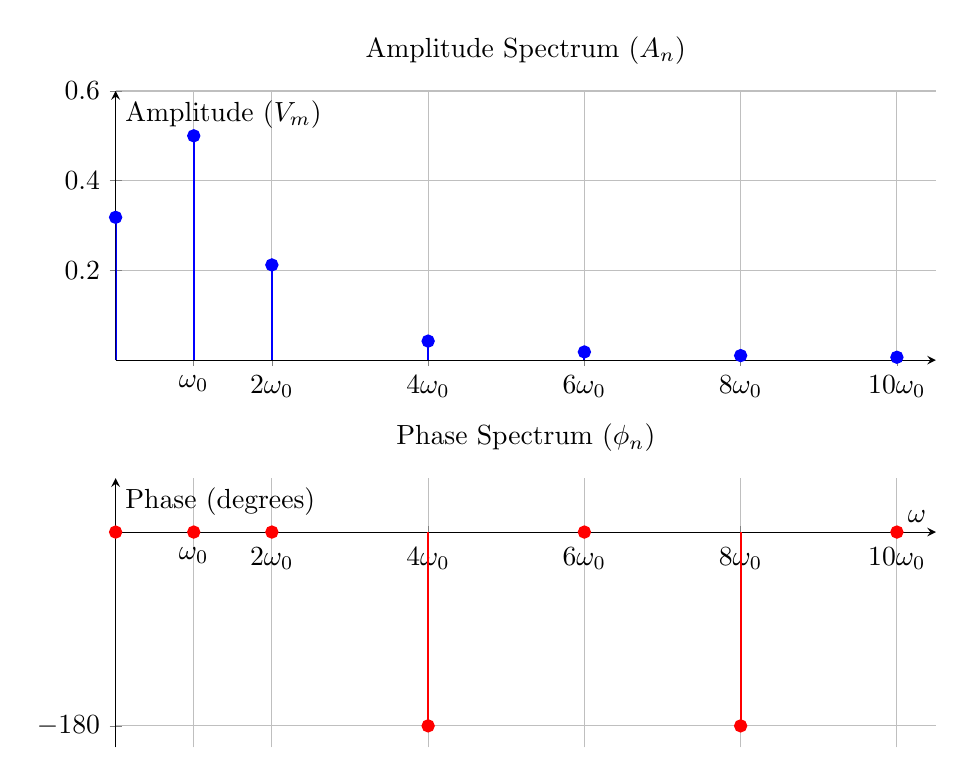
\begin{tikzpicture}
    \begin{groupplot}[
        group style={
            group size=1 by 2,
            vertical sep=1.5cm,
            xlabels at=edge bottom
        },
        width=12cm, height=5cm,
        axis lines=middle,
        xlabel={$\omega$}, 
        xmin=0, xmax=6.5,
        xtick={0,1,2,4,6},
        xticklabels={0, $\omega_0$, $2\omega_0$, $4\omega_0$, $6\omega_0$},
        grid=both,
        ymin=0
    ]
    
    % Amplitude Spectrum (An)
    \nextgroupplot[title={Amplitude Spectrum ($A_n$)}, ylabel={Amplitude ($V_m$)}, ymax=0.6, xmin=0, xmax=10.5, xtick={0,1,2,4,6,8,10}, xticklabels={0, $\omega_0$, $2\omega_0$, $4\omega_0$, $6\omega_0$, $8\omega_0$, $10\omega_0$}]
        \addplot[blue, mark=*, ycomb, thick] coordinates {
            (0, 0.3183)   % DC: 1/pi
            (1, 0.5)      % n=1: 1/2
            (2, 0.2122)   % n=2: 2/(3pi)
            (4, 0.0424)   % n=4: 2/(15pi)
            (6, 0.0182)   % n=6: 2/(35pi)
            (8, 0.0101)   % n=8: 2/(63pi)
            (10, 0.0064)  % n=10: 2/(99pi)
        };

    % Phase Spectrum (phi_n)
    \nextgroupplot[title={Phase Spectrum ($\phi_n$)}, ylabel={Phase (degrees)}, ymin=-200, ymax=50, ytick={0, -180}, xmin=0, xmax=10.5, xtick={0,1,2,4,6,8,10}, xticklabels={0, $\omega_0$, $2\omega_0$, $4\omega_0$, $6\omega_0$, $8\omega_0$, $10\omega_0$}]
        \addplot[red, mark=*, ycomb, thick] coordinates {
            (0, 0)
            (1, 0)
            (2, 0)
            (4, -180)     % n=4 term is negative
            (6, 0)        % n=6 term is positive
            (8, -180)     % n=8 term is negative
            (10, 0)       % n=10 term is positive
        };

    \end{groupplot}
\end{tikzpicture}
\end{document}
